\section{Mehrelektronensysteme}
\subsection{Paulisches Ausschließungsprinzip}
Ausschließungsprinzip: zwei Elektronen in einem Atom können nicht in allen Quantenzahlen übereinstimmen.
$\rightarrow$ Spins in gleichen Orbitalen sind antiparallel.

Bei entarteten Sternen: gilt Pauli für ein Phasenraumvolumen $dr^3 \cdot dp^3 \, = \, h^3$.

\subsection{Beschreibung von Zuständen}
\begin{equation*}
	n^{2S+1}L_j
\end{equation*}
\begin{itemize}
	\item $L = \sum l, \; S = \sum s$: Gesamtbahndrehimpuls / Spin
	\item ($2S + 1$): Spin-Multiplizität (Anzahl Einstellmöglichkeiten für Gesamtspin)
\end{itemize}
Pauli: $S = 0$ für $L = 0$ (S-Orbital)

\subsection{Kopplung von Drehimpulsen}
\begin{center}
	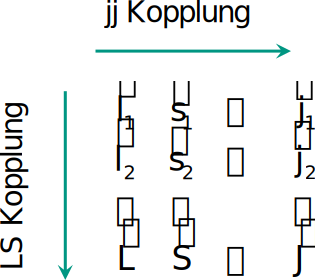
\includegraphics[width=.25\textwidth]{img/ls-jj-coupling.pdf}
\end{center}

\subsubsection{Russel-Saunders ($LS$)-Kopplung}
Tritt bei kleinen Kernen ($Z < 30$) auf.

\[\vec{S} = \sum \vec{s}, \quad \vec{L} = \sum \vec{l}, \quad \vec{J} = \vec{L} + \vec{S}\]

Quantisierung bei zwei Elektronen ($\vec{l_1}$ und $\vec{l_2}$ nicht parallel): \[L = l_1 - l_2 \dots l_1 + l_2 \; (l_1 > l_2)\]

$\rightarrow$ $L=0$: S-Term, $L=1$: P-Term, $L=2$: D-Term.
\subsubsection{$jj$-Kopplung}

\subsection{Madelung Schema}
\begin{center}
\includegraphics[width=.25\textwidth]{img/madelung-rule.pdf}
\end{center}
In den jeweiligen Grundzuständen der Atome werden nach aufsteigendem $(n + l)$, zweitrangig nach aufsteigendem $n$ aufgefüllt.
Es gibt allerdings auch Ausnahmen wie zB. Chrom: \textmath{[Ar] 3d^5 4s^1}.
